\section{Analysis Procedure}
The main objective of the HF sourcing analysis is to transfer the HF energy
calibration used in Run I to the new hardware to be used during Run II. More
specifically, it is to compute calibration coefficients (so called "HF
Gains", not to be confused with PMT gains), validate them, and upload the
results to the offline database for further use. All the data files
collected during these campaigns are stored on disk at CERN in the EOS
storage system.

The general content of the data files is reduced to include pertenant
information for calibration, such as the indexes of each channel powered
during the campaign, a two-dimensional array containing each channel's
output signal and capacitor ID (CapID), the name of the source tube being
sourced during any given event, the position of the radioactive source
with respect to the source driver, etc. The reduced data file is still
substantially large given that many wedges were connected to power during
each campaign, each providing output signals for its 24 towers at two
channels per tower (EM or H).

The output (EM and H channels) from the tower containing the
radioactive source are considered signal data, while the background data
is collected for each tower while the radioactive source is sufficiently
far away. To gaurantee that the radioactive source is sufficeintly distant
from a given tower measuring background data, the following requirements for each tower's $\eta$ index (IEta) for a wedge half with a given $\phi$ index (IPhi) were considered:
\begin{center}
   \begin{eqnarray}
      \label{eq:Tower_Cuts}
      \textrm{Source in IEta = 29: Record Background for IEta $\ge$ 34,} \\
      \textrm{Source in IEta = 39: Record Background for IEta $<$ 34.} \nonumber
   \end{eqnarray}
\end{center}

Therefore, for a given channel within a given tower and wedge, signal and background data are colleceted separately based on the location of the
radioactive source described above. Provided that histograms for each channel
are being read out by the DAQ at a rate of every four events, and each event
contains all four capacitors' histograms for each QIE. Loop over all
events recorded for a given channel and sum together all four capacitors'
histograms. To eliminate extraneous data resulting from energy deposition
in the optical fiber bundles as the radioactive source has yet to fully
penetrate the absorber, restrict the loop over events when source is positioned strictly inside of the calorimeter: [start + 300 mm, end - 300 mm],
where start and end are the distances from the source driver at
which the given source tube begins and ends within the absorber, respectively.
The reason to also exclude data when the radioactive source nears the Tube End
position is due to extraneous data resulting from some optical fibers extending
beyond the length of the absorber. This tail end cut also helps in unifying
signal data definitions between the EM and H channels, given that the H fibers
are shorter in length than the EM fibers.

In combining the histograms from all four capacitors within an event, one can
then study the newly constructed total histogram as a function of reel position
of the radioactive source within the absorber - this ability is crucial for
radiation damage studies within the HF calorimeters. However, for the intent of
calibrating the new PMTs installed for Run II, the choice is made to focus on comparing the total energy deposition recorded within a given tower with the expected energy deposition provided from the radioactive source. Therefore, we constuct a 32 bin histogram, with similar ADC charge bin ranges as provided by the firmware, that stores the overall sum of all events' 4-capacitor histograms according to the following:
\begin{center}
   \begin{equation}
      \label{eq:Histo_Sum}
      N_j = \sum\limits_{i=l}^m \sum\limits_{CapID=1}^4 n_j
   \end{equation}
\end{center}

where $N_j$ and $n_j$ are the content of the $j^{th}$ bin of their respective
histograms, and $i$ is the event with $l$ and $m$ restricted according to
go only over events with souce position within the tower as defined previously.

The mean ADC charge is defined separately for signal and background data of a
particular tower by averaging over the bins of the total histogram from all
events,
\begin{center}
   \begin{eqnarray}
      \label{eq:Histo_Avg}
      \langle{Q}\rangle = (\frac{1}{N} \sum\limits_{j=1}^{31} N_{j}q_{j}) - P, \\
      N = \sum\limits_{j=1}^{31} N_j \nonumber
   \end{eqnarray}
\end{center}

where $\langle{Q}\rangle$ is the mean ADC charge for the total histogram,
$N$ is the total number of entries within the bin range [1,31], $q_j$ is
the central ADC charge for the $j^{th}$ bin, and $P$ is the Gaussian mean of
the pedestal region. All sourcing histograms have a clear feature of a pedestal
peak. That is due to the fact that there is no actual trigger during
histogramming mode. Every TS data gets recorded. Therefore the number of events
that fall under the pedestal is several orders of magnitude larger than in the
beyond pedestal region, and the $\mu$ and $\sigma$ of the pedestal are dominated
by histogram's mean and width. The charge due to pedestal, $P$, is computed by fitting the histogram within the pedestal region [$\mu$ - 4$\sigma$, $\mu$ + 4$\sigma$] (if lower bound falls below 0, take 0 as the min value) with a Gaussian function and extracting the function's mean.

To determine the charge deposition for a given channel of a tower,
${\langle{Q}\rangle}_c$~, the background mean ADC
charge, ${\langle{Q}\rangle}^{(b)}_{c}$, must be subtracted from the signal yield,
${\langle{Q}\rangle}^{(s)}_{c}$, as follows:
\begin{center}
   \begin{equation}
      \label{eq:Sig_Min_Bkg}
      {\langle{Q}\rangle}_{c} = {\langle{Q}\rangle}^{(s)}_{c} - {\langle{Q}\rangle}^{(b)}_{c}.
   \end{equation}
\end{center}

To account for energy leakage, due to the restraints on geometric
containment of the radiated energy from the radioactive source within the tower,
the geometric correction factors must be applied, $G_c$~, listed in
Table~\ref{tab:hf_description_gcfactors} as follows:
\begin{center}
   \begin{equation}
      \label{eq:Sig_Corr}
      {\langle{Q}\rangle}^{Geom}_{c} = \frac{{\langle{Q}\rangle}_{c}}{G_{c}}\unit{ADC/25ns}.
   \end{equation}
\end{center}

Up to this point, the analysis procedure was identical for both 2013 and 2014
Sourcing Campaigns. However, to proceed further with calibration (calculating the
actual HF Gains), the source energy deposition had to be extracted from 2013 data.

\subsection{Extracting Source Energy Deposition}
The source energy deposition is the amount of energy deposited by the source in
units of GeV/25 ns. The actual source signal is measured (computed) in
ADC/25 ns. Therefore, a conversion factor GeV/ADC, which comes from
Run I Conditions, is needed. To extract Run I HF Gains and QIE Slopes from the Conditions DataBase (CondDB), we used Run 203777. Since 2013 sourcing was performed with the old PMTs, the
Calibration Coefficients ${CC}^{Run I}_{c}$~ (GeV/ADC) used during Run I were used to convert
the signal measured in ADC/25\unit{ns} into GeV/25\unit{ns}. It is important to point out that in calculation of energy deposition, response corrections are not included. That is because the Run I calibration for PMT gains should be preserved, when extracting the energy, but not the HF response, which is affected by other corrections accumulated in response corrections.

In figure~\ref{fig:QIE_Slope}, correlation plots between the inverted Calibration
Coefficients (ADC/GeV) from Run I and Source Signal (ADC/25\unit{ns}) from 2013
Campaign are presented. Here, a similar strategy to Run I Calibration was used, when
EM and HAD channels were calibrated separately. Except for some outlier channels,
we observe a good correlation between Signals collected (in 2013) and the Run I
Calibration Constants. Therefore, we can extract Source Energy Deposition:
\begin{center}
	\begin{equation}
		\label{eq:Edep}
		{\langle{E}\rangle}_{c} = {\langle{Q}\rangle}^{Geom}_{c} \times {CC^{Run I}_{c}}.
	\end{equation}
\end{center}

\begin{figure}[htb]
   \begin{center}
      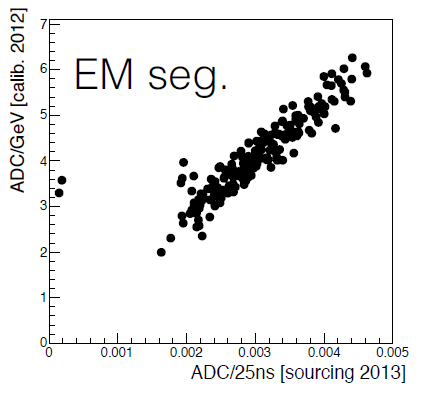
\includegraphics[width=.45\textwidth]{figures/ch_hfcalibration/QIE_Res_EM.png}
      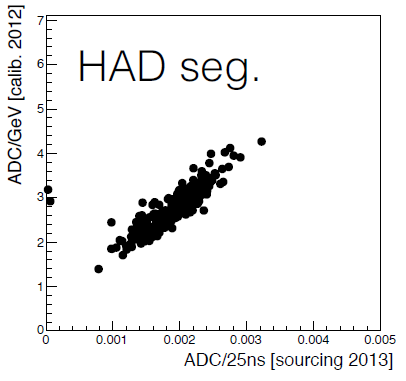
\includegraphics[width=.45\textwidth]{figures/ch_hfcalibration/QIE_Res_H.png}
      \caption{(a) Correlation plot between QIE response, in ADC/GeV, and 2013 HF-
               geometry corrected energy deposition, in ADC/25\unit{ns}, per tower
               for the EM channel.
               (b) Similar correlation is observed for the H channel.}
      \label{fig:QIE_Slope}
   \end{center}
\end{figure}

\subsection{Calculating Calibration Coefficients}
During Run II, HF will be operated at the Operational Voltage 2 (OV2). Since
both 2014 sourcing campaigns were done at voltage settings, OV1 and OV1+100,
different from the one to be used, the actual source signals should be converted to
the desired voltage, by using gains for the respective voltages. Another factor to
account for is the firmware setting, either 1 TS or 2 TS. Taking these 2 arguments
into account, compute a source signal at OV2 in units of ADC/25\unit{ns}:
\begin{center}
	\begin{equation}
		\label{eq:Sig_OV2}
		{\langle{Q}\rangle}^{Geom,OV2}_{c} = \frac{{\langle{Q}\rangle}^{Geom}_{c}}{nTS} \times \frac{{GAIN}^{OV2}}{{GAIN}^{OV1,OV1+100}}.
	\end{equation}
\end{center}
Finally, compute the actual Calibration Coefficients (HF Gains) ${CC}^{Run II}_{c}$:
\begin{center}
	\begin{equation}
		\label{eq:HF_Gains}
		{CC}^{Run II}_{c} = \tau \times \frac{{\langle{E}\rangle}^{2013}}{{\langle{Q}\rangle}^{Geom, OV2}_{c}}.
	\end{equation}
\end{center}
where $\tau$ is the source radioactivity correction factor, which accounts for exponential source activity decrease. We take 2013 sourcing date as the starting point and compute the decrease for April and July 2014 with respect to that date.
